\documentclass[a4paper,12pt]{article}

\usepackage[utf8]{inputenc}
\usepackage[left=0.5in,right=0.5in,top=1in,bottom=1in]{geometry}
\usepackage{amsmath,amssymb,amsfonts}
\usepackage{pgfplots,graphicx,calc,changepage}
\pgfplotsset{compat=newest}
\usepackage{enumitem}
\usepackage{fancyhdr}
\usepackage[colorlinks = true, linkcolor = blue]{hyperref}

% Syntax highlighting
\usepackage{listings}
\usepackage{xcolor}

\definecolor{codegreen}{rgb}{0.40,0.62,0.07}
\definecolor{codegray}{rgb}{0.5,0.5,0.5}
\definecolor{codeblue}{rgb}{0.09,0.57,0.73}
\definecolor{backcolour}{rgb}{1,1,1}

\lstdefinestyle{mystyle}{
    backgroundcolor=\color{backcolour},   
    commentstyle=\color{codegreen},
    keywordstyle=\color{magenta},
    numberstyle=\tiny\color{codegray},
    stringstyle=\color{codeblue},
    basicstyle=\ttfamily\small,
    breaklines=true,                     
    keepspaces=true,                 
    numbers=left,                    
    numbersep=5pt,                  
    showspaces=false,
    showstringspaces=false,
    showtabs=false,                  
    tabsize=4
}

\lstset{style=mystyle}

\newcommand{\nats}{\mathbb{N}}
\newcommand{\reals}{\mathbb{R}}
\newcommand{\rats}{\mathbb{Q}}
\newcommand{\ints}{\mathbb{Z}}
\newcommand{\comps}{\mathbb{C}}
\newcommand{\pols}{\mathcal{P}}
\newcommand{\cants}{\Delta\!\!\!\!\Delta}
\newcommand{\eps}{\varepsilon}
\newcommand{\st}{\backepsilon}
\newcommand{\abs}[1]{\left| #1 \right|}
\newcommand{\dom}[1]{\mathrm{dom}\left(#1\right)}
\newcommand{\for}{\text{ for }}
\newcommand{\dd}[1]{\mathrm{d}#1}
\newcommand{\spn}{\mathrm{sp}}
\newcommand{\nul}{\mathcal{N}}
\newcommand{\col}{\mathrm{col}}
\newcommand{\rank}{\mathrm{rank}}
\newcommand{\norm}[1]{\lVert #1 \rVert}
\newcommand{\inner}[1]{\left\langle #1 \right\rangle}
\newcommand{\pmat}[1]{\begin{pmatrix} #1 \end{pmatrix}}
\renewcommand{\and}{\text{ and }}

\newsavebox{\qed}
\newenvironment{proof}[2][$\square$]
    {\setlength{\parskip}{0pt}\par\textit{Proof:} #2\setlength{\parskip}{0.25cm}
        \savebox{\qed}{#1}
        \begin{adjustwidth}{\widthof{Proof:}}{}
    }
    {
        \hfill\usebox{\qed}\end{adjustwidth}
    }

\pagestyle{fancy}
\fancyhead{}
\lhead{Caleb Jacobs}
\chead{APPM 5600: Numerical Analysis I}
\rhead{Homework \#7}
\cfoot{}
\setlength{\headheight}{35pt}
\setlength{\parskip}{0.25cm}
\setlength{\parindent}{0pt}

\begin{document}
\section*{Problems}
	\begin{enumerate}[label = \arabic*)]
		\item We want to construct a rational function of the form
		\[
			R(z) = \frac{\alpha + \beta z}{1 + \gamma z}
		\]
		that interpolates the data $ (z_1, f_1), (z_2, f_2), (z_3, f_3) $ at distinct points $ z_1, z_2,  $ and $ z_3 $. In other words, we seek $ \alpha, \beta, $ and $ \gamma $ such that 
		\[
			R(z_j) = f_j, \quad j=1,2,3.
		\]
		Show how you can determine $ \alpha, \beta, $ and $ \gamma $ by setting a linear system $ Ax = b $ for the unknown vector $ x = (\alpha, \beta, \gamma)^T $.
		
		First, we need 
		\[
			R(z_i) = \frac{\alpha + \beta z_i}{1 + \gamma z_i} =  f_i
		\]
		which implies
		\begin{align*}
			& \alpha + \beta z_i = f_i + \gamma f_i z_i \\
			\implies & \alpha + \beta z_i - \gamma f_i z_i = f_i
		\end{align*}
		for $ i = 1,2, 3 $. We can rewrite this system as
		\[
			\pmat{1 & z_1 & -f_1 z_1 \\ 1 & z_2 & -f_2 z_2 \\ 1 & z_3 & -f_3 z_3} \pmat{\alpha \\ \beta \\ \gamma} = \pmat{f_1 \\ f_2 \\ f_3}.
		\]
		Solving this system will give us the desired $ \alpha, \beta, $ and $ \gamma $.
		
		\item We studied in class interpolation of functions defined in 1D. We can adapt the technique to higher dimensions. For instance, let
		\[
			f(x,y) = e^x \sin(y).
		\]
		We want to construct a polynomial of the form
		\[
			p(x,y) = c_0 + c_1x + c_2 y + c_3 xy + c_4 x^2 + c_5 y^2
		\]
		that interpolates $ f $ at the points $ (x_i, y_i) $:
		\begin{equation}
			p(x_i,y_i) = f(x_i, y_i); \quad i = 1, \ldots, 5. \label{equ:pol}
		\end{equation}
		
		\begin{enumerate}[label = (\roman*)]
			\item Set up a linear system $ Ac = f $ to determine the coefficients $ c_0, \ldots, c_5 $.
			
			Using \eqref{equ:pol}, we obtain the linear system:
			\[
				\pmat{
					1 & 0 & 0 & 0 & 0 & 0 \\
					1 & 0 & 2 & 0 & 0 & 4 \\
					1 & 1 & 0 & 0 & 1 & 0 \\
					1 & 1 & 2 & 2 & 1 & 4 \\
					1 & 2 & 1 & 2 & 4 & 1 \\
					1 & 2 & 3 & 6 & 4 & 9
				} \pmat{
					c_0 \\ c_1 \\ c_2 \\ c_3 \\ c_4 \\ c_5 
				} = \pmat{e^0 \sin(0) \\ e^0 \sin(2) \\ e^1 \sin(0) \\ e^1 \sin(2) \\ e^2 \sin(1) \\ e^2 \sin(3)}.
			\]
			
			\item Write a MATLAB code to determine $ c $ when the data points are
			\[
				(0,0), (0,2), (1,0), (1,2), (2,1), (2,3)
			\]
			
			Using my code which is attached to the end of the PDF I obtained $ c $ as 
			\[
				c =
				\pmat{
					0 \\
					-9.491631052234917e-01 \\
					5.059193000070850e+00 \\
					7.812146225895686e-01 \\
					9.491631052234921e-01 \\
					-2.302272143329005e+00
				}.
			\]
			
			\item Plot your polynomial $ p $ over $ x \in [-1,3], y \in [-1,3] $. Compare this plot to the similar plot for $ f $.
			
			\begin{figure}[h!]
				\centering
				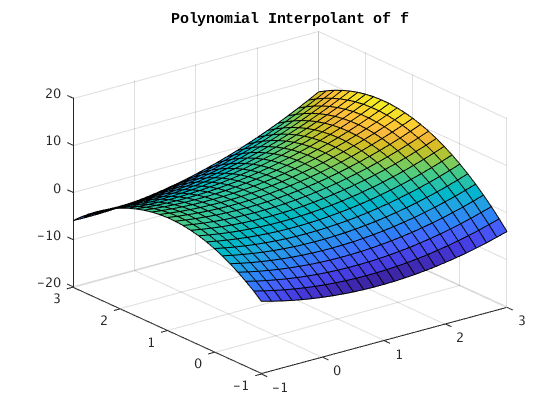
\includegraphics[width = 0.45\textwidth]{images/PolF.png}
				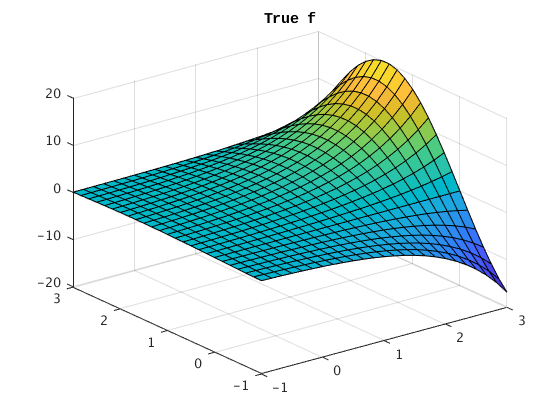
\includegraphics[width = 0.45\textwidth]{images/TrueF.png}
				\caption{\emph{Left}:Polynomial interpolant of $ e^x \sin(y) $. \emph{Right}: $ e^x \sin(y) $}
				\label{fig:pol}			
			\end{figure}
		
			From Figure \ref{fig:pol}, we can see that our interpolant is similar in the middle of the plot. However, once we get near the boundaries of our plots, the accuracy of our interpolant degrades significantly (eyeball norm shows a difference). The degradation near the boundaries is due to the data not being given at the boundaries of our plot and so we are extrapolating. Likewise, the middle of the interpolant is relatively accurate because we have data points near the middle. 
		\end{enumerate}
	
		\item Recall the Lagrange basis functions $ L_j (x) $ are defined by
		\[
			L_j(x) = \prod_{i \neq j} \left(\frac{x - x_i}{x_j - x_i}\right)
		\]
		for $ \{x_i\}_{i=1}^n $.
		
		\begin{enumerate}[label = (\roman*)]
			\item Prove that for any $ n \geq 1 $,
			\[
				\sum_{j = 0}^{n} L_i(x) = 1
			\]
			for all $ x \in \reals $.
			
			\begin{proof}{}
				Suppose we are creating an nth degree interpolating polynomial of the function $ f(x) = 1 $ over the data points $ x_0, x_1, \ldots, x_n $ using Lagrange polynomials. Then our polynomial would be given by
				\[
					p(x) = \sum_{j = 0}^n (1) L_j (x) = \sum_{j = 0}^n L_j(x).
				\]
				Then, because $ f(x) = 1 $ is a 0th degree polynomial and because polynomial interpolants are unique for any given set of data points, $ p(x) = 1 $. Therefore
				\[
					p(x) = \sum_{j = 0}^n L_j(x) = 1.
				\]
			\end{proof}
			
			\item Define $ \Psi(x) K (x - x_0) \cdots (x - x_n) $. Show that the polynomial interpolant of degree n that interpolates the data $ (x_i, f(x_i)) $ for $ i = 0, \ldots, n $ can be written in the form 
			\[
				p_n(x) = \sum_{i=0}^{n} \frac{\Psi(x)}{(x - x_i) \Psi'(x_i)} f(x_i)
			\]
			provided $ x \neq x_i $ for all $ i $.
			
			To show our equality, we first need to compute the first derivative of $ \Psi(x) $ as
			\begin{align*}
				\frac{\dd}{\dd x} \Psi(x) &= \frac{\dd}{\dd x} \prod_{j= 0}^{n} (x - x_j) \\
				&= \sum_{k = 0}^n \prod_{j \neq k} (x - x_j).
			\end{align*}
			Then, evaluating $ \Psi'(x) $ at $ x = x_i $ for $ i = 0, \ldots, n $, we have
			\begin{align*}
				\Psi'(x_i) &= \sum_{k = 0}^n \prod_{j \neq k} (x_i - x_j) \\
				&= \prod_{i \neq j}(x_i - x_j) \quad \text{from the product rule.}
			\end{align*}
			Next, using the Lagrange basis and with $ x \neq  x_i $ for each $ i $, we can form the nth degree interpolating polynomial of our data with
			\begin{align*}
				p_n(x) &= \sum_{i = 0}^{n} f(x_i) L_i(x) \\
				&= \sum_{i = 0}^{n} \frac{x - x_i}{x - x_i} f(x_i) L_i(x) \\
				&= \sum_{i = 0}^{n} \frac{x - x_i}{x - x_i} f(x_i) \prod_{i \neq j} \frac{x - x_j}{x_i - x_j} \\
				&= \sum_{i = 0}^{n} \left(\frac{1}{x - x_i} \prod_{i \neq j} \frac{1}{x_i - x_j} \right)  \left((x - x_i)\prod_{i \neq j} (x - x_j)\right) f(x_i) \\
				&= \sum_{i = 0}^{n} \left(\frac{1}{(x - x_i) \Psi'(x_i)}\right)  \left(\prod_{j = 0}^n (x - x_j)\right) f(x_i) \\
				&= \sum_{i = 0}^{n} \left(\frac{1}{(x - x_i) \Psi'(x_i)}\right)  \left(\Psi(x)\right) f(x_i) \\
				&= \sum_{i = 0}^n \frac{\Psi(x)}{(x - x_i) \Psi'(x_i)} f(x_i).
			\end{align*}
		
			\newpage
			\item Define next
			\[
				w_i = \frac{1}{\Psi'(x_i)}.
			\]
			Show that the polynomial interpolant of degree $ n $ that interpolates the data $ (x_i, f(x_i)) $ for $ i = 0, \ldots, n $ can be written in the form
			\[
				p_n(x) = \frac{\sum_{i = 0}^{n} \frac{w_i f(x_i)}{x - x_i}}{\sum_{i = 0}^{n} \frac{w_i}{x - x_i}}
			\]
			provided $ x \neq x_i $ for all $ i $.
			
			First, let's rewrite $ \Psi(x) $ using our result from part (i):
			\begin{align*}
				\Psi(x) &= \prod_{i = 0}^{n} (x - x_i) / 1 \\
				&= \prod_{i = 0}^{n} (x - x_i) \frac{1}{\sum_{j = 0}^{n} L_j(x)} \\
				&= \frac{1}{\prod_{i = 0}^{n} \frac{1}{x - x_i}} \frac{1}{\sum_{j = 0}^{n} L_j(x)} \\
				&= \frac{1}{\sum_{j = 0}^n \left(\prod_{i = 0}^{n} \frac{1}{x - x_i}\right)L_j(x)} \\
				&= \frac{1}{\sum_{j = 0}^n\left(\prod_{i = 0}^{n} \frac{1}{x - x_i}\right) \left(\prod_{k \neq j}\frac{x - x_k}{x_j - x_k}\right)} \\
				&= \frac{1}{\sum_{j = 0}^n\left(\prod_{i = 0}^{n} \frac{1}{x - x_i}\right) \left(\prod_{k \neq j}(x - x_k)\right) w_j} \\
				&= \frac{1}{\sum_{j = 0}^n \frac{1}{x - x_j} w_j} \\
				&= \frac{1}{\sum_{j = 0}^n \frac{w_j}{x - x_j}}
			\end{align*}
			
			
			Finally, using our results from the previous line and part (ii), we have
			\begin{align*}
				p_n(x) &= \sum_{i = 0}^n \frac{\Psi(x)}{(x - x_i) \Psi'(x_i)} f(x_i) \\
				&= \sum_{i = 0}^n w_i \frac{\Psi(x)}{(x - x_i)} f(x_i) \\
				&= \Psi(x) \sum_{i = 0}^n \frac{w_i f(x_i)}{(x - x_i)} \\
				&= \frac{1}{\sum_{i = 0}^n \frac{w_i}{x - x_i}} \sum_{i = 0}^n \frac{w_i f(x_i)}{(x - x_i)} \\
				&= \frac{\sum_{i = 0}^{n} \frac{w_i f(x_i)}{x - x_i}}{\sum_{i = 0}^{n} \frac{w_i}{x - x_i}}.
			\end{align*}
		\end{enumerate}
	\end{enumerate}

\section*{Code Used}
	\lstinputlisting[language = matlab]{code/Problem_2.m}
\end{document}